\if0
☆レポート課題(チームで一部だけ提出して下さい)

1. 表紙(課題名、チームメンバ氏名、提出日)

2. SingleCycleMIPSのモジュール仕様書
 設計した各モジュールについて、上位階層から順に、下記の内容をまとめること。
 ・モジュール名
 ・モジュールの入出力信号名とその説明

例: 入力信号一覧
name 	width 	explanation
CLK 	[0:0] 	SingleCycleMIPS用クロック信号
PC 	[31:0] 	次に実行する命令アドレスを格納するレジスタ値


 ・モジュール内のブロック図(サブモジュール間の接続関係を明示すること。ただし、最下層のIF, ID, EX, MAについては、ブロック図は不要です。)
 ・モジュールの動作の説明文

3. 実機DE10-Liteでの動作検証
 ・テストプログラムのファイル名一覧(load_store, arithmetic, array, if_then_else, while, function, recursion, hanoi)
 ・テストプログラムの実行方法
 ・テストプログラムの検証法
 ・各テストプログラムの検証結果

4. 考察(メンバ一人づつ、個別の考察を記述して下さい。1600文字以上/人)
 ・今回の回路設計で工夫した点(技術的な視点、チーム内での役割分担等のプロジェクト管理的な視点)
 ・より実用的なMIPSプロセッサを実現するために、マイクロアーキテクチャの観点から改良すべき点、および、それに関連して追加で実装すべき機能/回路

5. 感想(メンバ一人づつ、個別の感想を記述して下さい。800文字程度)

6.参考文献
\fi
\documentclass[dvipdfmx]{jsarticle}
\usepackage{graphicx}[dvipdfmx]
\usepackage{multirow}
\usepackage{array}
\usepackage{amsmath,amssymb}
\usepackage{url}
\usepackage{listings}
\usepackage{color}
\usepackage{verbatim}

\title{計算機設計論 レポート課題:MIPSプロセッサの回路設計}
\author{1295149 森岡悠人\\}
\date{\today}

\begin{document}
\maketitle

\section{モジュール仕様書}


QuartusのRTL Viewerを用いて出力した,DE10-liteに書き込んだモジュールのブロック図を図\ref{fig:rtl}に示す.
\begin{figure}[h]
\centering
  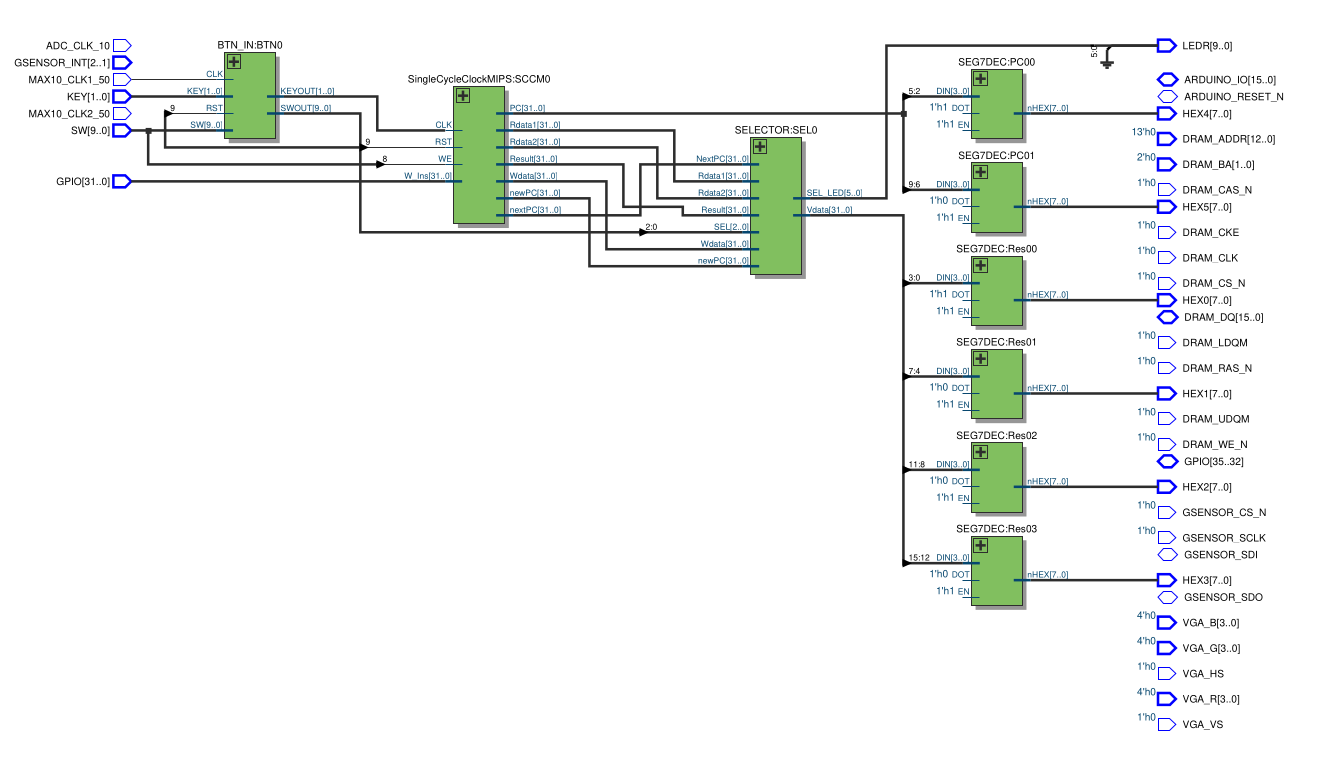
\includegraphics[width=\textwidth]{myRTL.png}
  \caption{作成したMIPS回路のブロック図}
  \label{fig:rtl}
\end{figure}

\section{動作検証}
作成したverilogコードがMIPSの命令セットを実行できるかどうかの検証を行った.
教科書\cite{textbook}に掲載されているアセンブラプログラム(load\_store, arithmetic, array, if\_then\_else, while, function, recursion, hanoi)を\texttt{IMem.txt}に書き込んでおき,IMに読み込ませ,modelsimを用いて動作のシミュレーションを行った.
シミュレーション結果は,display命令を用いて,PC, Instruction, ALU\_resultレジスタの内容を表示することで確認した.
シミュレーションには,modelsim 20.1を使用した.
シミュレーションの様子を図\ref{fig:simulation}に示す.

\begin{figure}[h]
\centering
  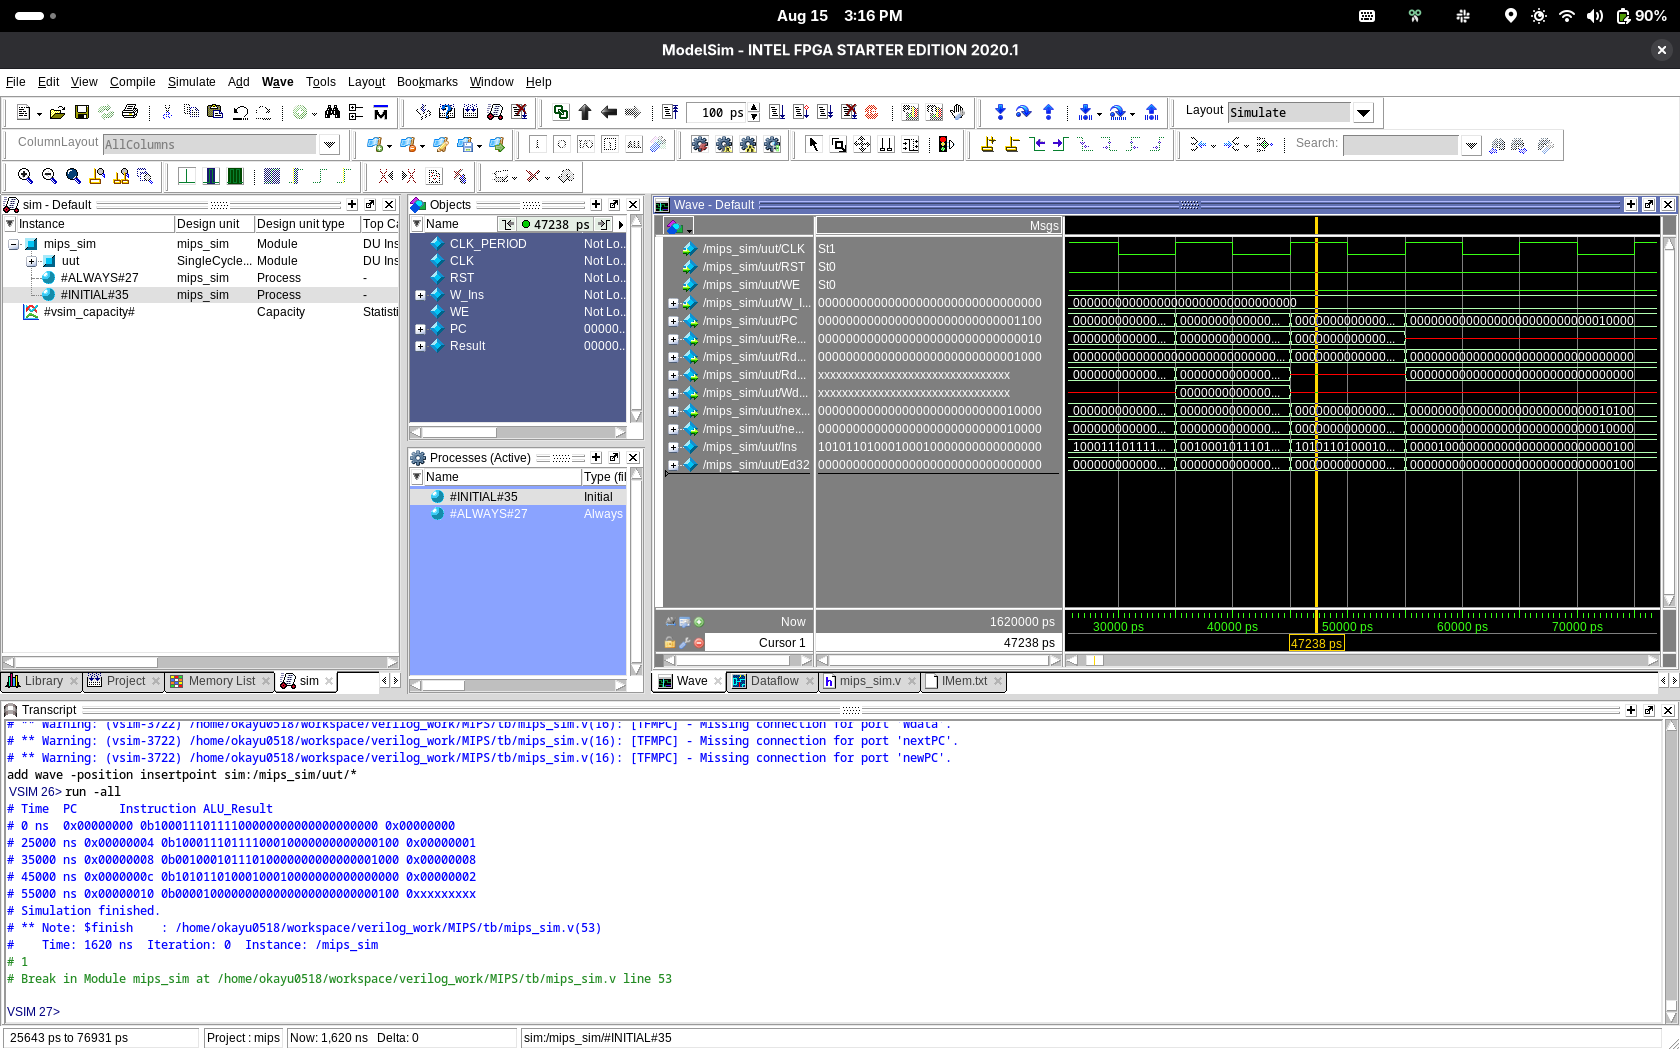
\includegraphics[width=0.8\textwidth]{modelsim.png}
  \caption{modelsimによるシミュレーションの様子}
  \label{fig:simulation}
\end{figure}

\subsection{test: load\_store}
\subsubsection{load\_storeのテスト結果}
\verbatiminput{test-results/load_store.txt}
\subsection{test: arithmetic}
\subsection{test: array}
\subsection{test: if\_then\_else}
\subsection{test: while}
\subsection{test: function}
\subsection{test: recursion}
\subsection{test: hanoi}


\section{考察}



\section{感想}



\bibliographystyle{junsrt}
\bibliography{refs}
\end{document}

